\section{Gráficos y análisis}

En esta parte del trabajo práctico se requiere determinar los enlaces transatlánticos que utiliza un paquete para llegar a destino. Estos enlaces se caracterizan por atravezar el Atlántico, por lo tanto poseen ciertas propiedades que los diferencian de los demás. Para poder detectar los posibles enlaces se utilizan las mediciones realizadas en la seeción anterior. A partir de los valores que se obtienen al ir recorriendo cada enlace por el que pasa una señal se puede determinar donde se encuentra el mayor salto.
Utilizandose el ZRTT calculado para cada salto se puede definir cuales son los valores que se encuentran más alejados del promedio, por lo tanto, aquellos que cumplan esa condición, serán los que representen el cambio de continente, habíendose atravezado el Atlántico.

Un ejemplo de cuando no funciona la metodología presentada, es aquel paquete que no utiliza por ningún enlace transatlántico. Determinaremos como trasatlánticos a aquel que no corresponda, ya que nos basamos en los tiempos transcurridos entre cada hops, por lo tanto no interesa si pasó o no por algún enlace específico.


\centerline{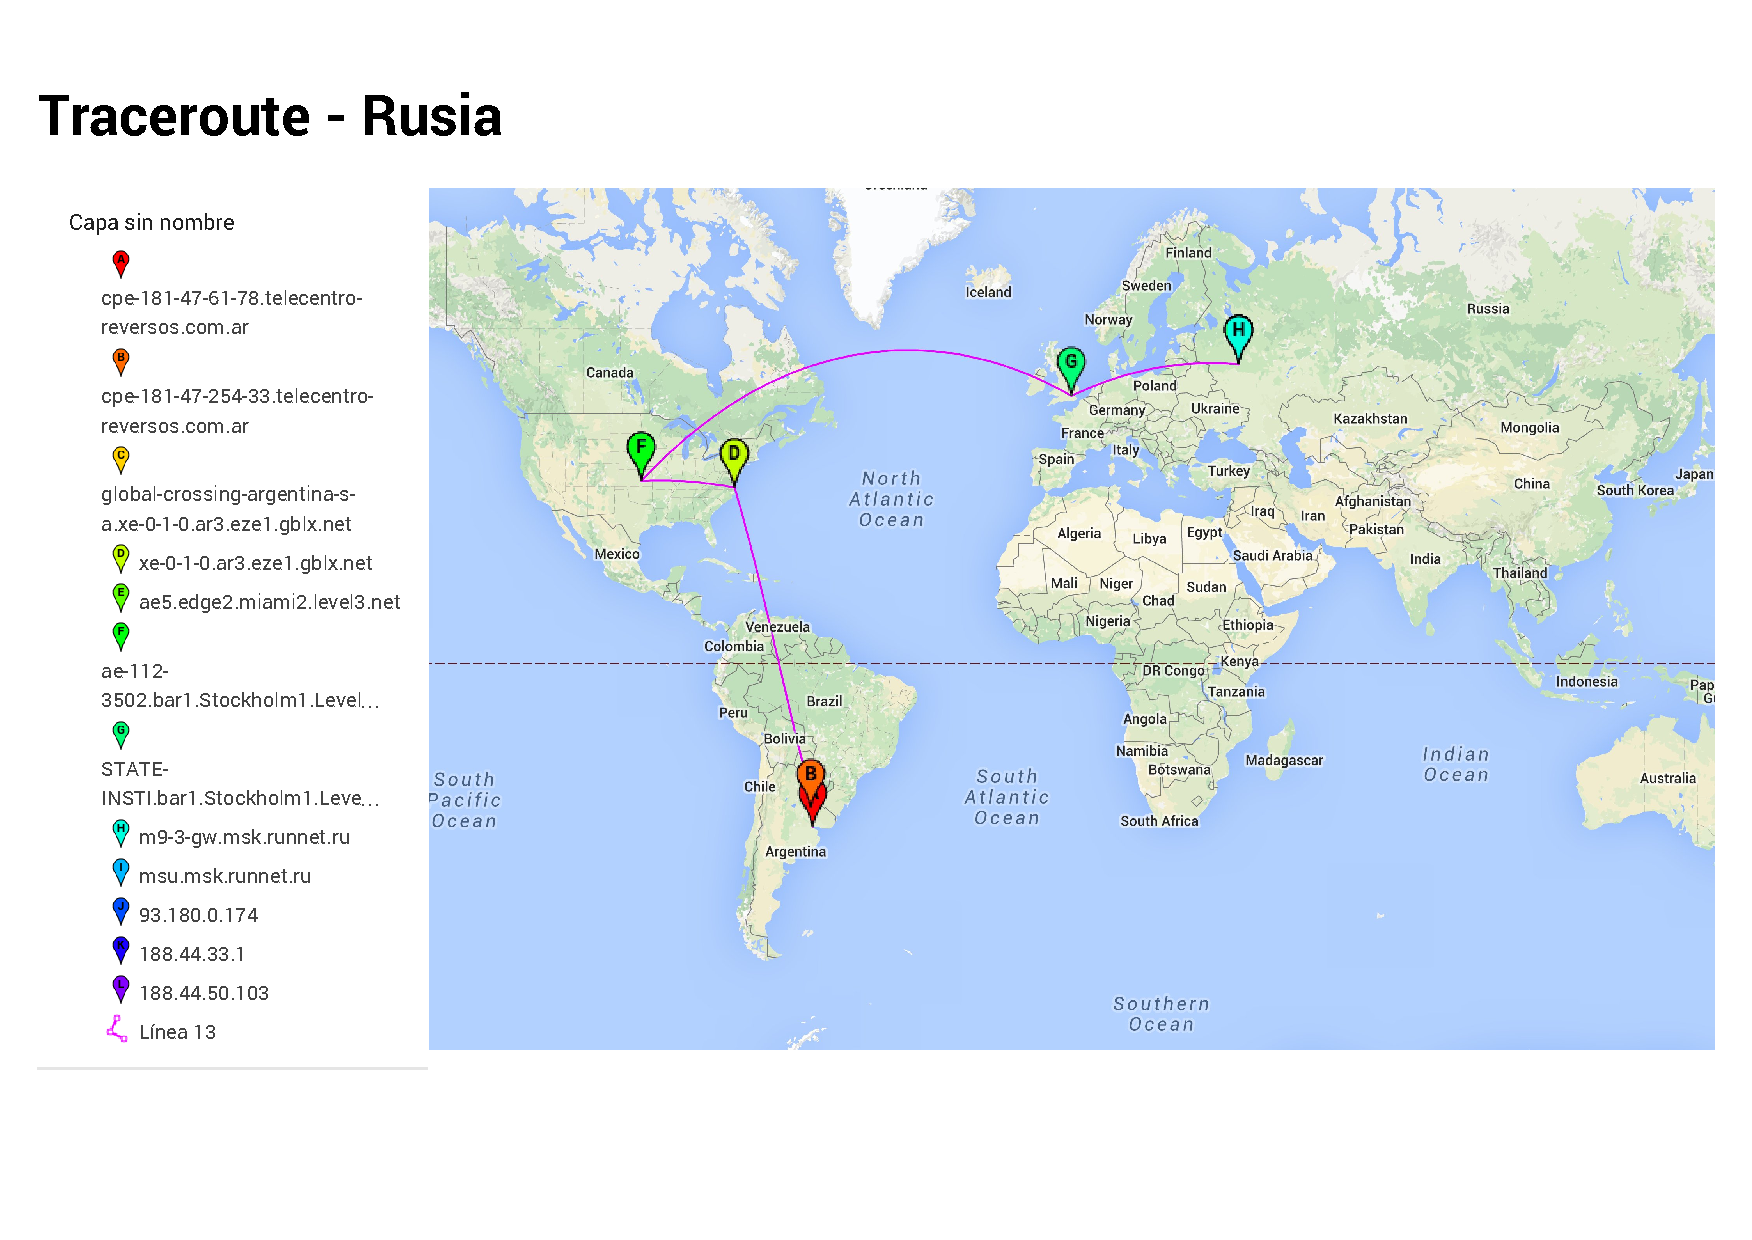
\includegraphics[width=0.8\textwidth]{mapas/rusia.png}}

\begin{center}
 \begin{tabular}{|l|l|l|l|l|}
    \hline
    Hop &Dirección IP &País &Ciudad &Lat - Long \\ \hline \hline
    1 &  & & & \\ \hline
    2 &  & & & \\ \hline
    3 &  & & & \\ \hline
    4 &  & & & \\ \hline
    5 &  & & & \\ \hline
    6 &  & & & \\ \hline
    7 &  & & & \\ \hline
    8 &  & & & \\ \hline
    9 &  & & & \\ \hline
    10 & & & & \\ \hline
    11 & & & & \\ \hline
    12 & & & & \\ \hline
    13 & & & & \\ \hline
    14 & & & & \\ \hline
    15 & & & & \\ \hline
    16 & & & & \\ \hline
    17 & & & & \\ \hline
 \end{tabular}
\end{center}

De acuerdo a la heurística desarrollada, el enlace trasatlántico se encuentra el marcador con la letra $CUAL$, y corresponde al que se encuentra entre el hop $NUMERO$ y el $NUMERO$.

\centerline{\includegraphics[width=0.8\textwidth]{mapas/Alemania.jpeg}}

\begin{center}
 \begin{tabular}{|l|l|l|l|l|}
    \hline
    Hop &Dirección IP &País &Ciudad &Lat - Long \\ \hline \hline
    1 & 190.190.247.1 & Argentina & Buenos Aires & -34.6 -58.5333	\\ \hline
    2 & 200.89.165.173 & Argentina & Buenos Aires & -34.6 -58.5333	\\ \hline
    3 & 200.89.165.130 & Argentina & Buenos Aires & -34.6 -58.5333	\\ \hline
    4 & 200.89.165.222 & Argentina & Buenos Aires & -34.6 -58.5333	\\ \hline
    5 & 208.178.195.205 & United States & Alexandria & 38.8048 -77.0469 \\ \hline
    6 & 67.17.75.66 & United States & - & 38.0 -97.0 \\ \hline
    7 & 4.68.111.121 & United States & - & 38.0 -97.0 \\ \hline
    8 & 4.68.111.121 & United States & - & 38.0 -97.0 \\ \hline
    9 & 4.69.154.137 & United States & - & 38.0 -97.0 \\ \hline
    10 & 212.162.4.6 & United Kingdom & - &  51.5 -0.13 \\ \hline
    11 & 188.1.144.101 & Germany & - & 51.0 9.0 \\ \hline
    12 & 188.1.144.185 & Germany & - & 51.0 9.0 \\ \hline
    13 & 188.1.144.158 & Germany & - & 51.0 9.0 \\ \hline
    14 & 188.1.144.13 & Germany & - & 51.0 9.0 \\ \hline
    15 & 188.1.144.17 & Germany & - & 51.0 9.0 \\ \hline
    16 & 188.1.236.70 & Germany & - & 51.0 9.0 \\ \hline
    17 & 141.20.0.210 & Germany & Berlin & 52.5167 13.4 \\ \hline
 \end{tabular}
\end{center}

En este caso se considera, observando el mapa, como enlace trasatlántico aquel que ocurre entre el hop $9$ y el $10$. Se puede observar en comparación con las variaciones de los valores de ZRTT, que el correspondiente al hop $10$, presenta un valor alto con respecto a los previos. Esto demuestra que el ZRTT es efectivo al momento de definir los saltos con cambios de continentes y que atraviezan el Atlántico.


\centerline{\includegraphics[width=0.8\textwidth]{mapas/Alemania.jpeg}}

\begin{center}
 \begin{tabular}{|l|l|l|l|l|}
    \hline
    Hop &Dirección IP &País &Ciudad &Lat - Long \\ \hline \hline
    1 &  & & & \\ \hline
    2 &  & & & \\ \hline
    3 &  & & & \\ \hline
    4 &  & & & \\ \hline
    5 &  & & & \\ \hline
    6 &  & & & \\ \hline
    7 &  & & & \\ \hline
    8 &  & & & \\ \hline
    9 &  & & & \\ \hline
    10 & & & & \\ \hline
    11 & & & & \\ \hline
    12 & & & & \\ \hline
    13 & & & & \\ \hline
    14 & & & & \\ \hline
    15 & & & & \\ \hline
    16 & & & & \\ \hline
    17 & & & & \\ \hline
 \end{tabular}
\end{center}

\centerline{\includegraphics[width=0.8\textwidth]{mapas/Alemania.jpeg}}

\begin{center}
 \begin{tabular}{|l|l|l|l|l|}
    \hline
    Hop &Dirección IP &País &Ciudad &Lat - Long \\ \hline \hline
    1 &  & & & \\ \hline
    2 &  & & & \\ \hline
    3 &  & & & \\ \hline
    4 &  & & & \\ \hline
    5 &  & & & \\ \hline
    6 &  & & & \\ \hline
    7 &  & & & \\ \hline
    8 &  & & & \\ \hline
    9 &  & & & \\ \hline
    10 & & & & \\ \hline
    11 & & & & \\ \hline
    12 & & & & \\ \hline
    13 & & & & \\ \hline
    14 & & & & \\ \hline
    15 & & & & \\ \hline
    16 & & & & \\ \hline
    17 & & & & \\ \hline
 \end{tabular}
\end{center}


\begin{center}
 \begin{tabular}{|l|l|l|l|l|}
    \hline
    Hop &Dirección IP &País &Ciudad &Lat - Long \\ \hline \hline
    3 & 181.47.254.85 & cpe-181-47-254-85.telecentro-reversos.com.ar & Argentina  & AS27747 & Telecentro S.A. & -34.6033 -58.3817 \\ \hline
    4 & 208.178.195.214 & global-crossing-argentina-s-a.xe-0-3-1.ar3.eze1.gblx.net & United States & Virginia AS3549 & Level 3 Communications, Inc. & 36.8267 -76.0179 \\ \hline
    5 & 208.178.195.213 & xe-0-3-1.ar3.eze1.gblx.net & United States & Virginia AS3549 & Level 3 Communications, Inc. & 36.8267 -76.0179 \\ \hline
    6 & 67.17.75.66 & po3-20G.ar3.MIA2.gblx.net & United States  & AS3549 & Level 3 Communications, Inc. & 38 -97 \\ \hline
    7 & 4.68.111.121 & ae5.edge2.miami2.level3.net & United States  & AS3356 & Level 3 Communications, Inc. & 38 -97 \\ \hline
    8 & 4.69.140.90 & ae-0-11.bar2.Boston1.Level3.net & United States & Florida AS3356 & Level 3 Communications, Inc. & 25.9372 -80.317 \\ \hline
    9 & 4.53.56.6 & BOSTON-UNIV.bar2.Boston1.Level3.net & United States & Massachusetts AS3356 & Level 3 Communications, Inc. & 42.2612 -71.4634 \\ \hline
    10 & 128.197.254.113 & comm595-core-aca01-gi2-16-comm595-bdr-gw01-gi1-2.bu.edu & United States & Massachusetts AS111 & Boston University & 42.3451 -71.0993 \\ \hline
    11 & 128.197.254.166 & cumm111-dist-aca01-te5-5-comm595-core-aca01-te3-1.bu.edu & United States & Massachusetts AS111 & Boston University & 42.3451 -71.0993 \\ \hline
    12 & 128.197.26.34 & www.bu.edu & United States & Massachusetts AS111 & Boston University & 42.3451 -71.0993 \\ \hline
 \end{tabular}
\end{center}
